\section{Comparación de Rendimiento}

\begin{frame}
    \frametitle{Resumen de Rendimiento: Éxito vs Fallo}

    \begin{columns}
        \column{0.48\textwidth}
        \begin{exampleblock}{Caso Exitoso: Paridad}
            \begin{itemize}
                \item \textbf{Reactive}: ~520ms
                \item \textbf{Structured}: ~520ms
                \item \textbf{Resultado}: Mismo rendimiento
            \end{itemize}
        \end{exampleblock}

        \begin{block}{¿Por qué iguales?}
            Ambos ejecutan todas las validaciones en paralelo y esperan que terminen
        \end{block}

        \column{0.48\textwidth}
        \begin{alertblock}{Caso Fallido: 60\% Más Rápido}
            \begin{itemize}
                \item \textbf{Reactive}: ~570ms
                \item \textbf{Structured}: ~230ms
                \item \textbf{Mejora}: \textcolor{red}{\textbf{60\%}}
            \end{itemize}
        \end{alertblock}

        \begin{block}{¿Por qué?}
            \begin{itemize}
                \item Reactive: allOf() espera TODAS
                \item Structured: Cancela automático
            \end{itemize}
        \end{block}
    \end{columns}

    \vspace{1em}
\end{frame}
\begin{frame}
    \begin{center}
        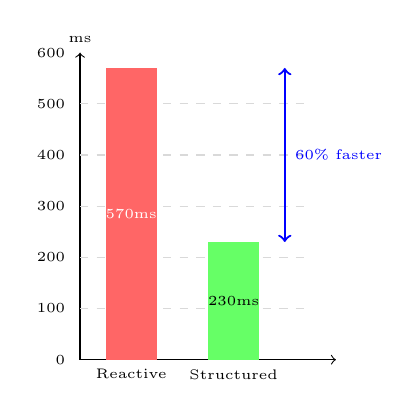
\begin{tikzpicture}[scale=0.65]
            % Y axis
            \draw[->] (0,0) -- (0,6) node[anchor=south] {\tiny ms};
            % X axis
            \draw[->] (0,0) -- (5,0);

            % Grid lines
            \foreach \y in {1,2,3,4,5}
                \draw[dashed, gray!30] (0,\y) -- (4.5,\y);

            % Y axis labels
            \node[anchor=east] at (-0.1,0) {\tiny 0};
            \node[anchor=east] at (-0.1,1) {\tiny 100};
            \node[anchor=east] at (-0.1,2) {\tiny 200};
            \node[anchor=east] at (-0.1,3) {\tiny 300};
            \node[anchor=east] at (-0.1,4) {\tiny 400};
            \node[anchor=east] at (-0.1,5) {\tiny 500};
            \node[anchor=east] at (-0.1,6) {\tiny 600};

            % Reactive bar (570ms ≈ 5.7 units)
            \fill[red!60] (0.5,0) rectangle (1.5,5.7);
            \node[anchor=north, font=\tiny] at (1,0) {Reactive};
            \node[font=\tiny, white] at (1,2.85) {570ms};

            % Structured bar (230ms ≈ 2.3 units)
            \fill[green!60] (2.5,0) rectangle (3.5,2.3);
            \node[anchor=north, font=\tiny] at (3,0) {Structured};
            \node[font=\tiny] at (3,1.15) {230ms};

            % Arrow showing difference
            \draw[<->, thick, blue] (4,2.3) -- (4,5.7) node[midway, right, font=\tiny] {60\% faster};

        \end{tikzpicture}
    \end{center}

    \begin{exampleblock}{Conclusi\'on}
        Mejor UX y menor uso de recursos en errores. 
        Mismo rendimiento en éxitos.
    \end{exampleblock}
\end{frame}

